\documentclass[a4paper]{report}
\input{../preamble.tex}
\title{Description Logic}

% account for different counting scheme in lecture
\counterwithout*{definition}{section}
\counterwithin*{definition}{chapter}
\renewcommand{\thedefinition}{\arabic{chapter}.\arabic{definition}}

% ensure right spacing around squared cup and cap
\let\helpercap\sqcap
\renewcommand{\sqcap}{\mathrel{\helpercap}}
\let\helpercup\sqcup
\renewcommand{\sqcup}{\mathrel{\helpercup}}

\begin{document}
	\selectlanguage{english}
	\maketitle
	\tableofcontents
	% TODO write Prolog containing reference to the book
	%% start of lectures
	% Chapter counting starts at 0
\setcounter{chapter}{-1}
\chapter{Introduction}
This is my transcript of the lecture "Description Logic" held by Prof. Dr. Franz Baader at TU Dresden in the summer semester 2021.
The lecture is based on the book "An Introduction to Description Logic" \cite{baader_dl_17} co-authored by Prof. Baader.

\chapter{Introduction}
\lecture{1}{18.04.2021}{}
Description Logic (DL) is a subfield of knowledge representation which intern is a subfield of Artificial Intelligence.
Note, that there is not \textbf{one} DL, but many different ones, most of which can be seen as fragments of FOL.
The general goal of Knowledge Representation and therefor of DL can be summarized as follows:
\begin{itemize}
	\item formalism: well-defined syntax and unambiguous semantics
	\item high-level description: only relevant aspects need to be represented
	\item intelligent applications: ability to infer implicit knowledge from the explicitly represented one
	\item effective: practical for reasoning tools and efficient implementable
\end{itemize}
Especially the latter point is interesting, since FOL is undecidable.
Therefore we must strike the right balance when it comes to expressive power.
Too low and not all the relevant knowledge can be presented, too high and reasoning becomes inefficient (or impossible).

The reasoning procedures used for processing the knowledge represented by a DL should satisfy the following properties:
\begin{itemize}
	\item soundness: Positive answers are indeed correct. 
	\item correctness: All positive answers are found, e.g.\ negative answers are correct.
	\item termination: There will always be an answer in finite time.
\end{itemize}
The procedure should furthermore be as efficient and as practical as possible.

To automatically reason about implicitly represented knowledge in a DL, one has to formalize the following:
\begin{itemize}
	\item syntax and semantics used in the DL (\textbf{description language}),
	\item the terminological knowledge of the application domain (\textbf{TBox}),
	\item the facts known about the specific "world" instance (\textbf{ABox}).
\end{itemize}

\chapter{A basic Description Logic}
In this chapter we will have a look at a basic DL called $\mathcal{ALC}$. 
The names of DLs follow a common naming scheme:
\begin{itemize}
	\item the basic language is called "attributive language"
	\item additional constructors are abbreviated with letters that are added after $ \mathcal{AL} $ 
	\item $ \mathcal{C} $ stands for \textit{complement}, i.e., $ \mathcal{ALC} $ is obtained from $ \mathcal{AL} $ by adding the complement ($ \neg $) operator
\end{itemize}

\section{The description language of $\mathcal{ALC}$}
\subsection{Syntax and semantics of $\mathcal{ALC}$}
\begin{definition}[Syntax of $\mathcal{ALC}$]
	Let $\mathscr{C}$ and $\mathscr{R}$ be disjoint sets of concept names and role names, respectively.
	$\mathcal{ALC}$-concept descriptions are inductively defined.
	\begin{itemize}
		\item If $ A \in \mathscr{C} $, then $ A $ is an $ \mathcal{ALC}$-concept description.
		\item If $ C,D $ are $ \mathcal{ALC}$-concept description, and $ r \in \mathscr{R} $, then the following are $\mathcal{ALC}$-concept descriptions:
			\begin{itemize}
				\item $ C \sqcap D $ (conjunction)
				\item $ C \sqcup D $ (disjunction)
				\item $ \neg C $ (negation)
				\item $ \forall r.C $ (value restriction)
				\item $ \exists r.C $ (existential restriction)
			\end{itemize}
	\end{itemize}
\end{definition}

\begin{note}
	One could equivalently define $\bot$ and $\top$ as concept descriptions.
	The main differences lie in the structure of induction proves and the length of formulas, that may be used in complexity analysis.
\end{note}

\begin{notation}
	We allow ourselves the use of parentheses for better structure and to define the following abbreviations:
	\begin{itemize}
		\item $ \top \coloneqq A \sqcup \neg A $ (top)
		\item $ \bot \coloneqq A \sqcap \neg A $ (bottom)
		\item $ C \Rightarrow D \coloneqq \neg C \sqcup D $ (implication)
	\end{itemize}
	Furthermore, we will use these conventions:
	\begin{itemize}
		\item Concept names are called \textit{atomic}.
		\item All other $\mathcal{ALC}$-concept descriptions are called \textit{complex}.
		\item We often abbreviate \textit{$\mathcal{ALC}$-concept description} with \textit{concept description} or just \textit{concept}.
		\item We often use $A, B$ for concept names, $C, D$ for (possibly) complex concepts and $r, s$ for role names.
		\item When talking about concrete elements of $\mathscr{C}$ or $\mathscr{R}$ we will use capitalized concept names and lowercased role names.
	\end{itemize}
\end{notation}

\begin{example}
	Here are some examples of the $\mathcal{ALC}$-syntax.
	Although the naming is chosen to have intuitive meaning, we have not defined a formal semantics of this description language yet.
	\begin{itemize}
		\item $ \var{Person} \sqcap \var{Female}$
		\item $ \var{Student} \sqcap \forall \var{attends}.(\var{Lecture}\sqcap \neg \var{Boring})$
	\end{itemize}
\end{example}

	\input{lec2.tex}
	\lecture{3}{20.04.2021}{}
\begin{example}
	Here is an example of an acyclic TBox:
	\begin{itemize}
		\item $ \var{Woman} \equiv \var{Person} \sqcap \var{Female}$
		\item $\var{Man} \equiv \var{Person} \sqcap \neg \var{Female}$
	\end{itemize}
	$\left\{ \var{Woman}, \var{Man} \right\} $ are the defined concepts and $\left\{ \var{Person}, \var{Female} \right\}$ are primitive concepts.
\end{example}

\begin{prop}
	For every acyclic TBox $\mathcal{T}$ we can effectively construct an equivalent acyclic TBox $ \widehat{\mathcal{T}}$
	such that the right-hand sides of concept definitions in $\widehat{\mathcal{T}}$ contain only primitive concepts.
\end{prop}
\begin{proof}
	By recursively expanding the (finitely many and acyclic) definitions.
\end{proof}

Given an acyclic TBox $\mathcal{T}$, a primitive interpretation $\mathcal{J}$ for $\mathcal{T}$ 
consists of a nonempty set $\Delta^{\mathcal{J}}$ together with an extension mapping $\cdot^{\mathcal{J}}$, that maps
\begin{itemize}
	\item primitive concepts $P$ to sets $P^{\mathcal{J}} \subseteq \Delta^{\mathcal{J}}$ 
	\item role names r to binary relations $r^\mathcal{J} \subseteq \Delta^{\mathcal{J}} \times \Delta^{\mathcal{J}}$
\end{itemize}
The interpretation $\mathcal{I}$ is an extension of the primitive interpretation $\mathcal{J}$ iff $\Delta^{\mathcal{J}} = \Delta^{\mathcal{I}}$ and
 \begin{itemize}
	\item $P^{\mathcal{J}} = P^{\mathcal{I}}$ for all primitive concepts $P$ 
	\item $r^{\mathcal{J}} = r^{\mathcal{I}}$ for all role names $r$
\end{itemize}

\begin{corollary}
	Let $\mathcal{T}$ be an acyclic TBox.
	Any primitive interpretation $\mathcal{J}$ for $\mathcal{T}$ has a unique extension to a model of $\mathcal{T}$.
\end{corollary}
\begin{proof}
	First construct the expanded TBox $\widehat{\mathcal{T}}$ for $\mathcal{T}$.
	Obviously, $\mathcal{T}$ and $\widehat{\mathcal{T}}$ have the same primitive and defined concepts.
	Let $\mathcal{J}$ be a primitive interpretation.
	We define its extension $\mathcal{I}$ as follows:
	For every defined concept $A$, let $A \equiv \hat{C}$ be its definition in $\widehat{\mathcal{T}}$.
	Since $\hat{C}$ contains only primitive concepts, $\hat{C}^{\mathcal{J}}$ is well-defined and we set $A^{\mathcal{I}} \coloneqq \hat{C}^{\mathcal{J}}$
	\begin{enumerate}
		\item $\mathcal{I}$ is a model of $\mathcal{T}$ : \newline
			By definition it is a model of $\widehat{\mathcal{T}}$ and we know $\mathcal{T}$ and $\widehat{\mathcal{T}}$ are equivalent.
		\item $\mathcal{I}$ is unique: \newline
			Assume that $\mathcal{I}'$ is another model of $\mathcal{T}$ that extends $\mathcal{J}$.
			Then $\mathcal{I}'$ is also a model of $\widehat{\mathcal{T}}$, and thus the following holds for all defined concepts $A$,
			where $A \equiv \hat{C}$ is the definition of $A$ in $\widehat{\mathcal{T}}$ :
			\[
				A^{\mathcal{I}'} = \hat{C}^{\mathcal{I}'} = \hat{C}^{\mathcal{J}} = \hat{C}^{\mathcal{I}} = A^{\mathcal{I}}
			. \qedhere \]
	\end{enumerate}
\end{proof}

\subsection*{Relationship with FOL}
$\mathcal{ALC}$-TBoxes can be translated into FOL:
\[
	\tau(\mathcal{T}) \coloneqq \bigwedge_{C \sqsubseteq D \in \mathcal{T}} \forall x.\left( \tau_x(C) \rightarrow \tau_x(D) \right)
.\]

\begin{lemma}
	Let $\mathcal{T}$ be a TBox, then $\mathcal{T}$ and $\tau(\mathcal{T})$ have the same models.
\end{lemma}
\begin{proof}
	trivial.
\end{proof}

\newpage
\section{Assertional knowledge}
\subsection{$\mathcal{ALC}$ ABoxes}
While concepts make statements about sets of individuals, we now want to state knowledge about specific individuals.

\begin{definition}[Assertions and ABoxes]
	An assertion is of the form $a:C$ (concept assertion) or $(a,b):r$ (role assertion),
	where $C$ is a concept description, $r$ is a role and $a,b$ are individual names from a set $\mathscr{I}$ of such names (disjoint with $\mathscr{C} \uplus \mathscr{R}$).
	An ABox is a finite set of assertions.
	An Interpretation $\mathcal{I}$ is a model of an ABox $\mathcal{A}$ if it satisfies all its assertions:
	\begin{itemize}
		\item $a^{\mathcal{I}} \in C^{\mathcal{I}}$ for all $a:C \in \mathcal{A}$ 
		\item $(a^{\mathcal{I}}, b^{\mathcal{I}}) \in r^{\mathcal{I}}$ for all $(a,b):r \in \mathcal{A}$
	\end{itemize}
\end{definition}

\begin{example}
	An example of an ABox:
	\begin{itemize}
		\item $ \var{MAX}: \var{Student}$
		\item $(\var{MAX}, \var{DL}): \var{interested}$
	\end{itemize}
\end{example}

\subsection{Relationship with FOL}
$\mathcal{ALC}$-ABoxes can be translated into FOL:
\[
	\tau(\mathcal{A}) \coloneqq \bigwedge_{a:C \in \mathcal{A}} \tau_{x}(C)(a) \land \bigwedge_{(a,b):r \in \mathcal{A}} r(a,b)
.\]

\begin{lemma}
	Let $\mathcal{A}$ be an ABox and $\tau(\mathcal{A})$ its translation into FOL.
	Then $\mathcal{A}$ and $\tau (\mathcal{A})$ have the same models.
\end{lemma}
\begin{proof}
	trivial.
\end{proof}

\newpage
\section{Knowledge Bases}
We will now combine the TBox and the ABox to form the foundation for reasoning in an DL.
\begin{definition}
	A knowledge base $\mathcal{K} = (\mathcal{T}, \mathcal{A})$ consists of a TBox $\mathcal{T}$ and an ABox $\mathcal{A}$.
	The interpretation $\mathcal{I}$ is a model of the knowledge base $\mathcal{K}$, iff it is a model of its TBox and its ABox.
\end{definition}
The FOL-translation of a knowledge base is easy, given its components:
\[
\tau(\mathcal{K}) \coloneqq \tau(\mathcal{T}) \land \tau(\mathcal{A})
.\] 
\begin{lemma}
	Let $\mathcal{K}$ be a knowledge base and $\tau(\mathcal{K})$ its translation into FOL.
	Then $\mathcal{K}$ and $\tau(\mathcal{K})$ have the same models.
\end{lemma}

\subsection{Additional constructors}
Individual names can also be used as concept constructors.
\begin{definition*}[$\mathcal{O}$ in the naming scheme.]
	This allows \textbf{nominals} $\left\{ a \right\} $ for $a \in \mathscr{I}$ with the semantics
	\[
	\left\{ a \right\} ^{\mathcal{I}} \coloneqq \left\{ a^{\mathcal{I}} \right\} 
	.\] 
	In this case, the ABox can be expressed using GCIs:
	\begin{itemize}
		\item $a:C$ is expressed as $\left\{ a \right\} \sqsubseteq C$
		\item $(a,b):r$ is expressed as $\left\{ a \right\} \sqsubseteq \exists r.\left\{ b \right\} $
	\end{itemize}
\end{definition*}

\newpage
\section{Reasoning Problems and Services}
\begin{definition}[terminological reasoning]
	Let $\mathcal{T}$ be a TBox and $C,D$ be (possibly) complex concept descriptions.
	We then consider the following decision problems:
	\begin{enumerate}
		\item Satisfiability: $C$ is satisfiable w.r.t.\ $\mathcal{T}$ iff
			$C^{\mathcal{I}} \neq \emptyset$ for some model $\mathcal{I}$ of $\mathcal{T}$.
		\item Subsumption: $C$ is subsumed by $D$ w.r.t.\ $\mathcal{T}$ $\left( C \sqsubseteq_{\mathcal{T}} D \right)$ iff
			$C^{\mathcal{I}} \subseteq D^{\mathcal{I}}$ for all models $\mathcal{I}$ of $\mathcal{T}$.
		\item Equivalence: $C$ is equivalent to $D$ w.r.t.\ $\mathcal{T}$ $\left( C \equiv_{\mathcal{T}} D \right) $ iff
			$C^{\mathcal{I}} = D^{\mathcal{I}}$ for all models $\mathcal{I}$ of $\mathcal{T}$.
		\item TBox consistency: $\mathcal{T}$ is consistent iff it has a model.
	\end{enumerate}
\end{definition}
\begin{notation}
	In the book a slightly different notation is used:
	\begin{itemize}
		\item $\mathcal{T} \vDash C \sqsubseteq D$ instead of $C \sqsubseteq_{\mathcal{T}} D$
		\item $\mathcal{T} \vDash C \equiv D$ instead of $C \equiv_{\mathcal{T}}D$
	\end{itemize}
\end{notation}
\begin{note}
	If $\mathcal{T} = \emptyset$, then satisfiability/subsumption/equivalence w.r.t.\ $\mathcal{T}$ is simply called satisfiability/subsumption/equivalence
	and we just write $\sqsubseteq$ and $\equiv$.	
\end{note}

\begin{example}
	Some examples:
	\begin{itemize}
		\item $A \sqcap \neg A$ and $\forall r.A \sqcap \exists r.\neg A$ are not satisfiable (unsatisfiable) \newline
			(therefore they are also equivalent and equivalent to $\bot$).
		\item $A \sqcap B$ is subsumed by $A$ and by $B$.
		\item $\exists r.(A \sqcap B)$ is subsumed by $\exists r.A$ and by $\exists r.B$
		\item $\forall r.(A \sqcap B)$ is equivalent to $\forall r.A  \sqcap \forall r.B$
	\end{itemize}
\end{example}

\begin{lemma}[Properties of subsumption]
	\begin{enumerate}
		\item The subsumption relation $\sqsubseteq_{\mathcal{T}}$ is a pre-order on concept descriptions, i.e.,
			\begin{itemize}
				\item $C \sqsubseteq_{\mathcal{T}}C$ (reflexive)
				\item $C \sqsubseteq_{\mathcal{T}} D \land D \sqsubseteq_{\mathcal{T}} E \implies C \sqsubseteq_{\mathcal{T}} E$ (transitive)
				\item It is however not antisymmetric in general and therefore not a partial order.
					This is because in general $C \sqsubseteq_{\mathcal{T}} D$ and $D \sqsubseteq_{\mathcal{T}} C$
					does imply $C \equiv_{\mathcal{T}} D$ but not necessarily $C = D$.
					They can be syntactically different descriptions for the same set.
			\end{itemize}
		\item The restriction constructors are monotonic w.r.t.\ subsumption, i.e.,
			\[
			C \sqsubseteq_{\mathcal{T}} D \implies \exists r.C \sqsubseteq_{\mathcal{T}} \exists r.D \text{ and } \forall r.C \sqsubseteq_{\mathcal{T}} \forall r.D
			.\] 
		\item Subsumption reasoning in monotonic, i.e., if $\mathcal{T} \subseteq  \mathcal{T}'$, then
			\[
				C \sqsubseteq_{\mathcal{T}} D \implies C \sqsubseteq_{\mathcal{T}'} D
			.\] 
	\end{enumerate}
\end{lemma}

	\lecture{4}{22.04.2021}{}
\begin{proof}
	\begin{enumerate}
		\item An easy consequence of the fact that $\subseteq$ on sets is reflexive and transitive.
		\item Assume that $C \sqsubseteq_{\mathcal{T}} D$.
			To show that $\forall r.C \sqsubseteq_{\mathcal{T}} \forall r.D$, we consider a model $\mathcal{I}$ of $\mathcal{T}$.
			We must show $ \left( \forall r.C \right)^{\mathcal{I}} \subseteq \left( \forall r.D \right)^{\mathcal{I}}$.
			Thus, let $d \in \left( \forall r.C \right)^{\mathcal{I}}$, i.e., for all $e \in \Delta^{\mathcal{I}}$,
			$\left( d,e \right) \in r^{\mathcal{I}} \implies e \in C^{\mathcal{I}}$.
			But then $C \sqsubseteq_{\mathcal{T}} D$ implies $C^{\mathcal{I}} \subseteq D^{\mathcal{I}}$.
			This yields $e \in D^{\mathcal{I}}$.
			Thus, $d \in \left( \forall r.C \right)^{\mathcal{I}}$.
			The proof for the existential restrictions is similar.
		\item Assume that $C \sqsubseteq_{\mathcal{T}} D$.
			Then, we have $C^{\mathcal{I}} \subseteq D^{\mathcal{I}}$ for all models $\mathcal{I}$ of $\mathcal{T}$.
			Let $\mathcal{T}'$ be such that $\mathcal{T} \subseteq \mathcal{T}'$.
			Then every model of $\mathcal{T}'$ is a model of $\mathcal{T}$.
			Thus, if $\mathcal{I}$ is a model of $\mathcal{T}'$, then $\mathcal{I}$ is a model of $\mathcal{T}$,
			and thus satisfies $C^{\mathcal{I}} \subseteq D^{\mathcal{I}}$.
			\qedhere
	\end{enumerate}
\end{proof}

\begin{lemma}[some basic equivalences]
	\begin{itemize}
		\item $\neg \top \equiv \bot$
		\item $C \sqcup D \equiv \neg \left( \neg C \sqcap \neg D \right)$
		\item $\forall r.C \equiv \neg \exists r.\neg C$
		\item $\exists r.\bot \equiv \bot$
		\item $\neg \left( \geq nr.C \right) \equiv \left( \leq n-1 r.C \right)$ if $n \geq 1$
		\item $\left( \geq 0 r.C \right) \equiv \top$
		\item $\left( \leq 0r.C \right) \equiv \forall r.\neg C$
	 \end{itemize}
\end{lemma}
\begin{proof}
	Lets have a closer look at $\forall r.C \equiv \neg \exists r.\neg C $.
	Let $\mathcal{I}$ be an interpretation.
	\begin{align*}
		d \in \left( \forall r.C \right)^{\mathcal{I}} & \iff \text{for all $e$ with $(d,e)\in r^{\mathcal{I}}$ we have $e \in C^{\mathcal{I}}$} \\
							& \iff \text{there is no $e$ with $(d,e)\in r^{\mathcal{I}}$ and $e \notin C^{\mathcal{I}}$} \\
							& \iff d  \notin \left( \exists r.\neg C \right)^{\mathcal{I}} \\
							& \iff d \in \left( \neg \exists r.(\neg C) \right)^{\mathcal{I}}
	\end{align*}
	Similar for the other equivalences. \qedhere
\end{proof}

\begin{definition}[assertional reasoning]
	Let $\mathcal{K} = \left( \mathcal{T}, \mathcal{A} \right)$ be a knowledge base, 
	$C$ a concept description and $a \in \mathscr{I}$.
	We then consider the following decision problems:
	\begin{enumerate}
		\item Knowledge base consistency: $\mathcal{K}$ is consistent iff there exists a model of $\mathcal{K}$.
		\item Instance: $a$ is an instance of $C$ w.r.t.\ $\mathcal{K}$ iff $a^{\mathcal{I}} \in C^{\mathcal{I}}$ 
			for all models $\mathcal{I}$ of $\mathcal{K}$.
	\end{enumerate}
\end{definition}
\begin{lemma}
	Let $\mathcal{K} = \left( \mathcal{T}, \mathcal{A} \right)$ be a knowledge base.
	If $a$ is an instance of $C$ w.r.t.\ $\mathcal{K}$ and $C \sqsubseteq_{\mathcal{T}} D$,
	then $a$ is an instance of $D$ w.r.t.\ $\mathcal{K}$.
\end{lemma}
\begin{proof}
	To Do !
\end{proof}

In the following we will show, that there exist certain polynomial reductions between the decision problems shown before:
\begin{figure}[H]
	\centering
	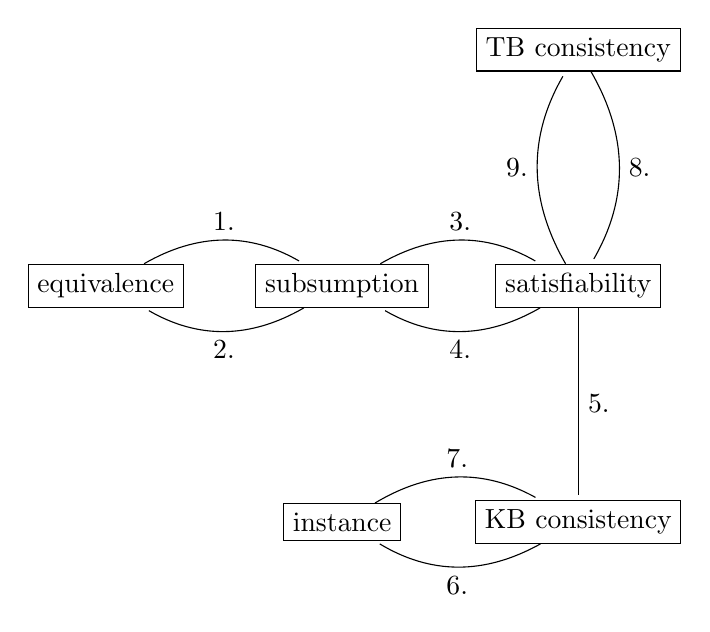
\begin{tikzpicture}[align=center,node distance=3cm, shorten >= 2pt]
		\node[draw] (eq) {equivalence};
		\node[draw, right of = eq] (sub) {subsumption};
		\node[draw, right of = sub] (sat) {satisfiability};
		\node[draw, below of = sat] (kbc) {KB consistency};
		\node[draw, left of = kbc] (ins) {instance};
		\node[draw, above of = sat] (tbc) {TB consistency};
		\draw (eq) edge[above, bend left] node{1.} (sub);
		\draw (sub) edge[below, bend left] node{2.} (eq);
		\draw (sub) edge[above, bend left] node{3.} (sat);
		\draw (sat) edge[below, bend left] node{4.} (sub);
		\draw (sat) edge[right]  node{5.} (kbc);
		\draw (kbc) edge[below, bend left] node{6.} (ins);
		\draw (ins) edge[above, bend left] node{7.} (kbc);
		\draw (tbc) edge[right, bend left] node{8.} (sat);
		\draw (sat) edge[left, bend left] node{9.} (tbc);
	\end{tikzpicture}
	\caption{Polynomial reductions between decision problems.}
	\label{fig:problem reductions}
\end{figure}
\begin{note}
	These reductions do not only hold for $\mathcal{ALC}$, but for all DLs with the constructors negation and conjunction.
	The last one also needs an existential quantifier.
	They correspond to the following lemma:
\end{note}

\begin{theorem}[polynomial reductions]
	Let $\mathcal{K} = \left( \mathcal{T}, \mathcal{A} \right)$ be a knowledge base, 
	$C, D$ concept descriptions and $a \in \mathscr{I}$.
	\begin{enumerate}
		\item $C \equiv_{\mathcal{T}} D \iff C \sqsubseteq_{\mathcal{T}} D \land D \sqsubseteq_{\mathcal{T}} C$ 
		\item $C \sqsubseteq_{\mathcal{T}} D \iff C \equiv_{\mathcal{T}} C \sqcap D$
		\item $C \sqsubseteq_{\mathcal{T}} D \iff C \sqcap \neg D$ is unsatisfiable w.r.t.\ $\mathcal{T}$
		\item $C$ is satisfiable w.r.t.\ $\mathcal{T} \iff C \not\sqsubseteq_{\mathcal{T}} \bot$
		\item $C$ is satisfiable w.r.t.\ $\mathcal{T} \iff \left( \mathcal{T}, \left\{ a:C \right\} \right)$ is consistent
		\item $a$ is an instance of $C$ w.r.t.\ $\mathcal{K} \iff \left( \mathcal{T}, \mathcal{A} \cup \left\{ a: \neg C \right\} \right)$ is inconsistent
		\item $\mathcal{K}$ is consistent $\iff a$ is not an instance of $\bot$ w.r.t.\ $\mathcal{K}$
		\item $\mathcal{T}$ is consistent $\iff \top$ is satisfiable w.r.t.\ $\mathcal{T}$
		\item $C$ is satisfiable w.r.t.\ $\mathcal{T} \iff \mathcal{T} \cup \left\{ \top \sqsubseteq \exists r.C \right\}$,
			where $r$ is a new role that does not occur in $C$ or $\mathcal{T}$,
			is consistent.
	\end{enumerate}
\end{theorem}
\begin{proof}
	\begin{enumerate}
		\item By definition.
		\item An easy consequence of the set inclusion relation $\subseteq$.
		\item
			\begin{align*}
				C \sqsubseteq_{\mathcal{T}} D & \iff \forall \mathcal{I}, \mathcal{I} \vDash \mathcal{T}: C^{\mathcal{I}} \subseteq D^{\mathcal{I}}\\
											  & \iff \forall \mathcal{I}, \mathcal{I} \vDash \mathcal{T} : C^\mathcal{I} \cap (\Delta^{\mathcal{I}} \setminus D^{\mathcal{I}}) = \emptyset\\
											  & \iff \forall \mathcal{I}, \mathcal{I} \vDash \mathcal{T}: C^{\mathcal{I}} \cap (\neg D)^\mathcal{I} = \emptyset\\
											  & \iff \forall \mathcal{I}, \mathcal{I} \vDash \mathcal{T}: \left( C \sqcap \neg D \right)^\mathcal{I} = \emptyset\\
											  & \iff \left( C \sqcap \neg D \right) \text{is unsatisfiable w.r.t.}\ \mathcal{T} 
			\end{align*}
		\item trivial.
		\item see lecture video.
		\item "$ \implies$": By its contraposition. \newline
			Assume that $\left( \mathcal{T}, \mathcal{A} \cup \left\{a: \neg C \right\} \right)$ is indeed consistent.
			Then there is  a model $\mathcal{I}$ of $\mathcal{T} , \mathcal{A}$ and $\left\{ a: \neg C \right\}$.
			But then $\mathcal{I}$ is a model of $\mathcal{K} = \left( \mathcal{T}, \mathcal{A} \right)$ such that
			$a^{\mathcal{I}} \notin C^\mathcal{I}$.
			Thus, $a$ is not an instance of $C$ w.r.t.\ $\mathcal{K}$. \newline
			"$\impliedby$": Also by its contraposition. \newline
			Assume that $a$ in not an instance of $C$ w.r.t.\ $\mathcal{K}$.
			Thus there is a model $\mathcal{I}$ of $\mathcal{K}$ with $a^\mathcal{I} \notin C^\mathcal{I}$.
			Thus, $\mathcal{I}$ is a model of $\left( \mathcal{T}, \mathcal{A} \cup \left\{ a: \neg C \right\} \right)$.
		\item By the contraposition: \newline
			Assume that $\mathcal{K}$ is consistent and let $\mathcal{I}$ be a model of $\mathcal{K}$.
			Then $a^\mathcal{I} \notin \emptyset = \bot^\mathcal{I}$.
			If $\mathcal{K}$ is inconsistent, then there is no model of $\mathcal{K}$.
			Thus $a^{\mathcal{I}} \in \bot^\mathcal{I}$ holds in all models since there are none.
		\item see lecture video.
		\item "$ \implies$": \newline
			Assume that $\mathcal{I}$ is a model of $\mathcal{T}$ such that $C^\mathcal{I} \neq \emptyset$
			(definition of satisfiability).
			Let $d \in C^{\mathcal{I}}$.
			We extend $\mathcal{I}$ to $\mathcal{I}'$by setting $r^{\mathcal{I}} = \left\{ (e,d) \mid  e \in \Delta^{\mathcal{I}} \right\}$.
			Since $r$ does not occur in $C$ or $\mathcal{T}$, we still have $d \in C^\mathcal{I'}$ and $\mathcal{I'}$ is a model of $\mathcal{T}$. \newline
			"$\impliedby$": \newline
			If $\mathcal{I}$ is a model of $\mathcal{T} \cup \left\{ \top \sqsubseteq \exists r.C \right\}$,
			then let $e$ be an arbitrary element of $\Delta^{\mathcal{I}}$.
			Then $e \in \left( \exists r.C \right)^{\mathcal{I}}$, and thus there is an $d \in \Delta^{\mathcal{I}}$ 
			with $\left( e,d \right) \in r^{\mathcal{I}}$ and $d \in C^\mathcal{I}$.
			Thus, $C$ is satisfiable w.r.t.\ $\mathcal{T}$.
			\qedhere
	\end{enumerate}
\end{proof}

Now we will show, that satisfiability w.r.t.\ $\mathcal{T}$ can be reduced to satisfiability (without $\mathcal{T}$) and
Knowledge base consistency can be reduced to ABox consistency.
However this reduction is in general not possible in polynomial time.

\begin{prop}[reductions to ABox consistency]
Let  $\mathcal{K} = (\mathcal{T}, \mathcal{A})$ be a knowledge base, where $\mathcal{T}$ is acyclic, and $C$ a concept description.
The expanded versions $\widehat{C}$ and $\widehat{A}$ of $C$ and $A$ w.r.t.\ $\mathcal{T}$ are obtained by
replacing all defined concepts occurring in $C$ and $A$ by their definitions in the expanded version $\widehat{\mathcal{T}}$ of $\mathcal{T}$.
Then:
	\begin{enumerate}
		\item $C$ is satisfiable w.r.t.\ $\mathcal{T} \iff \widehat{C}$ is satisfiable.
		\item $\mathcal{K} = (\mathcal{T},\mathcal{A})$ is consistent $\iff (\emptyset,\widehat{\mathcal{A}}$) is consistent.
	\end{enumerate}
\end{prop}
\begin{merke}[frametitle=Important Note:]
	The problem of deciding whether $(\emptyset, \widehat{\mathcal{A}})$ is consistent is also called "ABox consistency".
	The proposition above shows, that each of the decision problems discussed before can be reduce to ABox consistency,
	as long as no cyclic TBox is involved.
\end{merke}
\begin{proof}
	\begin{enumerate}
		\item " $\implies$":\newline
			Let $\mathcal{I}$ be a model of $\mathcal{T}$ with $C^\mathcal{I} \neq \emptyset$.
			Then $\mathcal{I}$ is also a model of $\widehat{\mathcal{T}}$ and we have $\emptyset \neq C^\mathcal{I} = \widehat{C}^\mathcal{I}$.
			Thus, $\widehat{C}$ is satisfiable. \newline
			"$\impliedby$": \newline
			Let $\mathcal{I}$ be an interpretation with $\widehat{C}^{\mathcal{I}} \neq \emptyset$.
			Let $\mathcal{J}$ be the primitive interpretation of which $\mathcal{I}$ is an extension
			and let $\mathcal{I}'$ be the model of $\mathcal{T}$ that extends $\mathcal{J}$.
			Since $\widehat{C}$ contains only primitive concepts,
			we have $\emptyset \neq \widehat{C}^{\mathcal{I}} = \widehat{C}^\mathcal{J} = \widehat{C}^{\mathcal{I'}} = C^{\mathcal{I'}}$,
			since $\mathcal{I}'$ is a model of $\mathcal{T}$ and $\widehat{\mathcal{T}}$.
		\item similar
			\qedhere
	\end{enumerate}
\end{proof}
\newpage

	\lecture{5}{27.04.2021}{}
So as long as we are not interested in the efficiency of reasoning, we do not need to develop reasoning procedures for TBoxes.
However, this reduction is in general not polynomial, since the expanded versions may be exponential in the size of $\mathcal{T}$.
One can easily see this with the following example on a TBox:
\begin{align*}
	A_0 &\equiv \forall r.A_1 \sqcap \forall s. A_1 \\
	A_1 &\equiv \forall r.A_2 \sqcap \forall s.A_2 \\
	\vdots & \\
	A_{n-1} & \equiv \forall r.A_n \sqcap \forall s.A_{n}
\end{align*}
The size of this TBox is linear in $n$,
but the expansion version $\widehat{A}_0$ of $A_0$ contains $A_n$ $2^n$ times.

\subsection{Relationship with FOL}
Like everything so far, reasoning in $\mathcal{ALC}$ can be translated into reasoning in FOL:
\begin{lemma}
	Let $\mathcal{K} = ( \mathcal{T},\mathcal{A})$ be a knowledge base, $C,D$ concept descriptions and $a$ an individual name.
	\begin{enumerate}
		\item $C \sqsubseteq_{\mathcal{T}} D \iff \tau(\mathcal{T}) \vDash \forall x.(\tau_x(C)(x) \Rightarrow \tau_x(D)(x))$
		\item $ \mathcal{K}$ is consistent $ \iff \tau(\mathcal{K})$ is consistent
		\item $a$ is an instance of $C$ w.r.t.\ $\mathcal{K} \iff \tau \left( \mathcal{K} \right) \vDash \tau_x(C)(a)$
	\end{enumerate}
\end{lemma}

\begin{proof}
	Exercise!	
\end{proof}

\newpage
\section{Further problems}
So far we have seen the basics of the $\mathcal{ALC}$-DL system and its inference problems.
Often times it is not sufficient to just know \textit{if} one concept is subsumed by another,
but which concepts are actually subsumed by which.
\textbf{Classification} is the task to compute the subsumption hierarchy of \textit{all} concept names occurring in the TBox.
\newline
Likewise, it could be of interest to know, which is the most specific concept name in the TBox to which an ABox individual belongs.
This problem is called \textbf{Realization}.
\newline
Therefore DL-systems often include solution procedures for these problems.

\section{Further relationships with FOL}
We will now introduce a new constructor for illustrative purposes.
If $r$ is a role name and $C$ is a concept description, then $\exists r^+.C $
is a concept description, with the semantics
\begin{align*}
	\begin{split}
		(\exists r^+.C)^\mathcal{I} \coloneqq &\left\{ d \in \Delta^{\mathcal{I}} \mid \exists n \geq 1, \exists d_1,\cdots, d_n \in \Delta^\mathcal{I} : \right.\\
											  &\left. (d,d_1) \in r^\mathcal{I}, \cdots, (d_{n-1},d_n) \in r^\mathcal{I} \land d_n \in C^\mathcal{I}\right\}
	\end{split}
\end{align*}

We claim, that $\exists r^+.C$ cannot be expressed in $\mathcal{ALC}$.
\begin{proof}
	Assume that there is an $\mathcal{ALC}$ concept $D$ such that $D \equiv \exists r^+.C$.
	Consider the ABox $\mathcal{A} = \left\{ a:D \right\}$.
	Let $ \mathcal{B} = \left\{ a : \forall r.\neg C, a: \forall r.\forall r.\neg C, a:\forall r.\forall r.\forall r.\neg C,\ldots \right\}$.
	Then $\mathcal{A} \cup \mathcal{B}$ is inconsistent.
	Since $\mathcal{A} \cup \mathcal{B}$ can be translated to FOL, compactness applies, i.e.,
	there is a finite subset $\mathcal{C} \subseteq \mathcal{A} \cup \mathcal{B}$ such that $\mathcal{C}$ is inconsistent.
	Let $n$ be the maximal nesting of value-restrictions in $\mathcal{C}$, i.e.,
	$\mathcal{C}$ does not contain $\underbrace{\forall r. \forall r. \ldots \forall r.}_{n+1} \neg C$.
	But then there obviously is a model of $\mathcal{C}$. $\contra$
\end{proof}
This shows, that certain concepts can be expressed in FOL, but not in $\mathcal{ALC}$.

\chapter{A Little Bit of Model Theory}
Like we already saw, interpretations of $\mathcal{ALC}$ can be viewed as graphs.
We introduce the notion of bisimulation between graphs and therefore between interpretations.
We will then show, that $\mathcal{ALC}$-concepts cannot distinguish bisimular nodes.
Afterwards these results will grant us the power to show restrictions of the expressive power of $\mathcal{ALC}$ and
interesting properties of models of $\mathcal{ALC}$:
\begin{itemize}
	\item tree model property
	\item closure under disjoint union
\end{itemize}
Furthermore we will show the very important property of $\mathcal{ALC}$: the finite model property.

\section{Bisimulation}
\begin{definition}[Bisimulation]\label{def:bisimulation}
	Let $\mathcal{I}_1$ and $\mathcal{I}_2$ be interpretations.
	The relation $\rho \subseteq \Delta^{\mathcal{I}_{1}} \times \Delta^{\mathcal{I}_2}$ is a bisimulation between $\mathcal{I}_1$ and $\mathcal{I}_2$ iff:
	\begin{enumerate}[label=(\roman*)]
		\item $d_1 \rho d_2 \implies d_1 \in A^{\mathcal{I}_1} \text{ iff } d_2 \in A^{\mathcal{I}_2}$ for all $A \in \mathscr{C}$
		\item $d_1 \rho d_2 \land  (d_1, d_1') \in r^{\mathcal{I}_1}$ implies the existence of $d_2' \in \Delta^{\mathcal{I}_2}$ such that
			$d_1' \rho d_2' \land (d_2, d_2') \in r^{\mathcal{I}_2}$ for all $r \in \mathscr{R}$
		\item $d_1 \rho d_2 \land  (d_2, d_2') \in r^{\mathcal{I}_2}$ implies the existence of $d_1' \in \Delta^{\mathcal{I}_1}$ such that
			$d_1' \rho d_2' \land (d_1, d_1') \in r^{\mathcal{I}_1}$ for all $r \in \mathscr{R}$
	\end{enumerate}
\end{definition}

\begin{note}
	\begin{itemize}
		\item $\mathcal{I}_1 = \mathcal{I}_2$ is possible
		\item the empty relation $\emptyset$ is always a bisimulation.
	\end{itemize}
\end{note}

\begin{notation}
	Let $\mathcal{I}_1, \mathcal{I}_2$ be interpretations and $d_1 \in \Delta^{\mathcal{I}_1}, d_2 \in \Delta^{\mathcal{I}_2}$.
	We then write:
	\[
		\left( \mathcal{I}_1, d_1 \right) \sim \left( \mathcal{I}_2, d_2 \right) \iff \exists \text{ a bisimulation $\rho$ between  $\mathcal{I}_1, \mathcal{I}_2$
		such that $d_1 \rho d_2$}
	.\]
	And we say "$d_1$ in $\mathcal{I}_1$ is bisimular to $d_2$ in $\mathcal{I}_2$".
\end{notation}

\begin{theorem}[Bisimulation invariance of $\mathcal{ALC}$]\label{thm: bisimulation invariance}
	If $ \left( \mathcal{I}_1,d_1 \right) \sim \left( \mathcal{I}_2, d_2 \right)$, then the following holds for all $\mathcal{ALC}$-concepts $C$ :
	\[
		d_1 \in C^{\mathcal{I}_1} \iff d_2 \in C^{\mathcal{I}_2}
	.\]
\end{theorem}
This theorem essentially tells us, that $\mathcal{ALC}$-concepts cannot distinguish between bisimular elements.

	\lecture{6}{29.04.2021}{}

\begin{proof}
	By induction on the structure of $C$ :
	\begin{itemize}
		\item $C = A \in \mathscr{C}$:
			Then $d_1 \in A^{\mathcal{I}_1}$ iff $d_2 \in A^{\mathcal{I}_2}$ is an immediate consequence of $d_1 \rho d_2$ for a bisimulation $\rho$.
		\item $C = D \sqcap E$ :
			$d_1 \in \left( D \sqcap E \right)^{\mathcal{I}_1}$ iff $d_1 \in D^{\mathcal{I}_1}$ and $d_1 \in E^{\mathcal{I}_1}$.
			But then $d_2 \in D^{\mathcal{I}_2}$ and $d_2 \in E^{\mathcal{I}_2}$ (induction).
			And therefore $d_2 \in \left( D \sqcap E \right)^{\mathcal{I}_2}$.
		\item $\neg, \sqcup$ can be treated similarly.
		\item $C = \exists r.D$ :
				$d_1 \in \left( \exists r.D \right)^{\mathcal{I}_1}$ iff there is $d_1' \in \Delta^{\mathcal{I}_1}$ such that $(d_1, d_1') \in r^{\mathcal{I}_1}$ and $d_1' \in D^{\mathcal{I}_1}$.
				Then there is $d_2' \in \Delta^{\mathcal{I}_2}$ such that $\left( d_2, d_2' \right) \in r^{\mathcal{I}_2}$ and $d_1' \rho d_2'$.
				By induction we get that $d_2' \in D^{\mathcal{I}_2}$ and therefore  $d_2 \in \left( \exists r.D \right)^{\mathcal{I}_2}$.
			\item $C = \forall r.D$ can be treated similarly.
	\end{itemize}
\end{proof}

\section{Expressive power}
We have so far introduced extensions of $\mathcal{ALC}$ by concept constructors \textbf{number restrictions}, \textbf{nominals} and the role constructor \textbf{invers roles}.
We will now show, that they really extend $\mathcal{ALC}$, i.e., there is no way these could be expressed by plain $\mathcal{ALC}$.

\begin{prop}[$\mathcal{ALCN}$ is more expressive than $\mathcal{ALC}$]
	No $\mathcal{ALC}$-concept description is equivalent to the $\mathcal{ALCN}$-concept description $\left( \leq 1 r \right)$.
\end{prop}
\begin{proof}
	Assume that $C$ is an $\mathcal{ALC}$-concept description such that $C \equiv ( \leq 1 r )$, i.e.\ $C^{\mathcal{I}} = \left( \leq 1 r \right)^\mathcal{I}$ holds for all interpretations $\mathcal{I}$.
	Consider the following two interpretations $\mathcal{I}_1$ and $\mathcal{I}_2$ :
	\begin{figure}[H]
		\centering
		\begin{subfigure}[t]{.475\textwidth}
			\centering
			\begin{tikzpicture}
				\node[default] (d1) {$d_1$};
				\node[default, below of = d1] (e1) {$e_1$};
				\draw (d1) edge[left] node{$r$} (e1);
			\end{tikzpicture}
			\caption{$\mathcal{I}_1$}
		\end{subfigure}
		\hfill
		\begin{subfigure}[t]{.475\textwidth}
			\centering
			\begin{tikzpicture}
				\node[default] (d2) {$d_2$};
				\node[default, below left of = d2] (e21) {$e_{2,1}$};
				\node[default, below right of = d2] (e22) {$e_{2,2}$};
				\draw (d2) edge[left] node{$r$} (e21);
				\draw (d2) edge[right] node{$r$} (e22);
			\end{tikzpicture}
			\caption{$\mathcal{I}_2$}
		\end{subfigure}
	\end{figure}
	Then $\rho \coloneqq \left\{ (d_1,d_2), (e_1,e_{2,1}), (e_1,e_{2,2}) \right\}$ is a bisimulation, which shows $(\mathcal{I}_1, d_1) \sim (\mathcal{I}_2,d_2)$.
	Thus, we have $d_1 \in C^{\mathcal{I}_1} \iff d_2 \in C^{\mathcal{I}_2}$.
	This yields a contradiction, since $d_1 \in ( \leq 1r)^{\mathcal{I}_1} = C^{\mathcal{I}_1}$ but $d_2 \notin ( \leq 1r)^{\mathcal{I}_2} = C^{\mathcal{I}_2}$. $\contra$
\end{proof}

\begin{prop}[$\mathcal{ALCI}$ is more expressive than $\mathcal{ALC}$]
	No $\mathcal{ALC}$-concept description is equivalent to the $\mathcal{ALCI}$-concept description $\exists r^{-}.\top$.
\end{prop}
\begin{proof}
	Assume that $C$ is an $\mathcal{ALC}$-concept description such that $C \equiv \exists r^{-}.\top$.
	Consider the following two interpretations:
	\begin{figure}[H]
		\centering
		\begin{subfigure}[t]{.475\textwidth}
			\centering
			\begin{tikzpicture}
				\node[default] (e1) {$e_1$};
				\node[default, below of = e1] (d1) {$d_1$};
				\draw (e1) edge[left] node{$r$} (d1);
			\end{tikzpicture}
			\caption{$\mathcal{I}_1$}
		\end{subfigure}
		\hfill
		\begin{subfigure}[t]{.475\textwidth}
			\centering
			\begin{tikzpicture}
				\node[default] (d2) {$d_2$};
			\end{tikzpicture}
			\caption{$\mathcal{I}_2$}
		\end{subfigure}
	\end{figure}
	Then $\rho \coloneqq \left\{ (d_1,d_2) \right\}$ is a bisimulation, which shows $\left(  \mathcal{I}_1, d_1 \right) \sim \left( \mathcal{I}_2,d_2 \right)$.
	Thus, we have  $d_1 \in C^{\mathcal{I}_1} \iff d_2 \in C^{\mathcal{I}_2}$.
	This yields a contradiction, since $d_1 \in \left( \exists r^{-}.\top \right)^{\mathcal{I}_1} = C^{\mathcal{I}_1}$, but
	$d_2 \notin \left( \exists r^{-}.\top \right)^{\mathcal{I}_2} = C^{\mathcal{I}_2}$. $\contra$
\end{proof}

\begin{prop}[$\mathcal{ALCO}$ is more expressive than $\mathcal{ALC}$]
	No $\mathcal{ALC}$-concept description is equivalent to the $\mathcal{ALCO}$-concept description $\left\{ a \right\}$.
\end{prop}
\begin{proof}
	Assume that $C$ is an $\mathcal{ALC}$-concept description such that $C \equiv \left\{ a \right\}$.
	Consider the following two interpretations:
	\begin{figure}[H]
		\centering
		\begin{subfigure}[t]{.475\textwidth}
			\centering
			\begin{tikzpicture}
				\node[default, label =left: $\left\{ a \right\}^{\mathcal{I}_1}$] (d1) {$d_1$};
			\end{tikzpicture}
			\caption{$\mathcal{I}_1$}
		\end{subfigure}
		\hfill
		\begin{subfigure}[t]{.475\textwidth}
			\centering
			\begin{tikzpicture}
				\node[default] (d2) {$d_2$};
				\node[default, label= right: $\left\{ a \right\}^{\mathcal{I}_2}$, right of = d2] (e2) {$e_2$};
			\end{tikzpicture}
			\caption{$\mathcal{I}_2$}
	\end{subfigure}
	\end{figure}
	The meaning of these interpretations is, that $a^{\mathcal{I}_1} = d_1$ and $a^{\mathcal{I}_2} = e_2$.
	Then $\rho \coloneqq \left\{ (d_1,d_2) \right\}$ is a bisimulation, which yields $\left( \mathcal{I}_1, d_1 \right) \sim \left( \mathcal{I}_2, d_2 \right)$.
	Thus, $d_1 \in C^{\mathcal{I}_1} \iff d_2 \in C^{\mathcal{I}_2}$.
	This yields a contradiction, since $d_1 \in \left\{ a \right\}^{\mathcal{I}_1} = C^{\mathcal{I}_1}$, but
	 $d_2 \notin \left\{ a \right\}^{\mathcal{I}_2} = C^{\mathcal{I}_2}$. $\contra$
\end{proof}
These proofs were the result of the fact, that we defined bisimulation with $\mathcal{ALC}$ in mind.
One could also define a notion of bisimulation under which $\mathcal{ALCN}$, $\mathcal{ALCI}$ or $\mathcal{ALCO}$ are invariant.

\section{Closure under disjoint union}
We will now introduce the notion of disjoint union for interpretations.
This will enable us to combine multiple interpretations into a bigger one, containing the interpretations it was built from,
but no interaction between them.
\begin{definition}
	Let $\mathfrak{R}$ be an index set and $\left( \mathcal{I}_{\nu} \right)_{\nu \in \mathfrak{R}}$ a family of interpretations $\mathcal{I}_{\nu} = \left( \Delta^{\mathcal{I}_{\nu}}, \cdot^{\mathcal{I}_{\nu}} \right)$.
	Their disjoint union $\mathcal{J}$ is defined as follows:
	\begin{align*}
		\Delta^{\mathcal{J}} &= \left\{ (d,\nu) \mid \nu \in \mathfrak{R}\land d \in \Delta^{\mathcal{I}_{\nu}} \right\}, \\
		A^{\mathcal{J}} &= \left\{ (d,\nu) \mid \nu \in \mathfrak{R} \land d \in A^{\mathcal{I}_\nu}\right\} \text{for all } A \in \mathscr{C}, \\
		r^{\mathcal{J}} &= \left\{ \left( (d,\nu),(e,\nu) \right) \mid \nu \in \mathfrak{R} \land (d,e) \in r^{\mathcal{I}_\nu} \right\} \text{for all } r \in \mathscr{R}.
	\end{align*}
\end{definition}
\begin{notation}
	We then write
	\[
	\mathcal{J} = \biguplus_{\nu \in \mathfrak{R}} \mathcal{I}_{\nu}
	.\]
\end{notation}
\begin{note}
	If there are some $\Delta^{\mathcal{I}_{\nu_1}}, \Delta^{\mathcal{I}_{\nu_2}}$ that are not disjoint,
	we make them artificially disjoint by adding the index $\nu$ to the tuple.
\end{note}

\begin{lemma}\label{lemma:disjoint union 1}
	For $\nu \in \mathfrak{R}$, all $\mathcal{ALC}$-concept description $C$, and all $d \in \Delta^{\mathcal{I}_\nu}$ we have:
	\[
		d \in C^{\mathcal{I}_\nu} \iff (d,\nu) \in C^{\mathcal{J}}
	,\]
	where $\mathcal{J} = \biguplus_{\nu \in \mathfrak{R}} \mathcal{I}_{\nu}$.
\end{lemma}
\begin{proof}[Proof sketch]
	Let $\mathcal{J} = \biguplus_{\nu \in \mathfrak{R}} \mathcal{I}_\nu$.
	We claim that
	\[
	\rho_\nu \coloneqq \left\{ \left( (d,\nu),d \right) \mid d \in \Delta^{\mathcal{I}_\nu} \right\}
	\]
	is a bisimulation (and proof that).
	And then lemma \ref{lemma:disjoint union 1} follows from theorem \ref{thm: bisimulation invariance}.
\end{proof}

\begin{theorem}\label{thm:disjoint union closure}
	Let $\mathcal{T}$ be an $\mathcal{ALC}$ TBox and $(\mathcal{I}_\nu)_{\nu \in \mathfrak{R}}$ a family of models of $\mathcal{T}$.
	Then its disjoint union $\mathcal{J} = \biguplus_{\nu \in \mathfrak{R}} \mathcal{I}_\nu$ is also a model of $\mathcal{T}$.
\end{theorem}
This theorem tells us, that models of TBoxes are closed under disjoint union.
\begin{proof}
	Let $C \sqsubseteq D \in \mathcal{T}$.
	We must show that $C^{\mathcal{J}} \subseteq D^{\mathcal{J}}$.
	Let $\left( d,\nu \right) \in C^{\mathcal{J}}$.
	By lemma \ref{lemma:disjoint union 1}, this implies $d \in C^{\mathcal{I}_\nu}$.
	Since $\mathcal{I}_\nu$ is a model of $\mathcal{T}$, we obtain $d \in D^{\mathcal{I}_\nu}$.
	Again, by lemma \ref{lemma:disjoint union 1}, this implies $(d,\nu) \in D^{\mathcal{J}}$.
\end{proof}

\begin{corollary}
 	Let $\mathcal{T}$ be an $\mathcal{ALC}$ TBox and $C$ an $\mathcal{ALC}$ concept that is satisfiable w.r.t.\ $\mathcal{T}$.
	Then there is a model $\mathcal{J}$ of $\mathcal{T}$ in which the extension $C^{\mathcal{J}}$ of $C$ is infinite.
\end{corollary}
\begin{proof}
	Since $C$ is satisfiable w.r.t.\ $\mathcal{T}$, there is a model $\mathcal{I}$ of $\mathcal{T}$ and $d \in \Delta^{\mathcal{I}}$ such that $d \in C^{\mathcal{I}}$.
	For $\nu \in \N^{+}$ let $\mathcal{I}_\nu = \mathcal{I}$.
	Let $\mathcal{J} = \biguplus_{\nu \geq 1} \mathcal{I}_\nu$.
	We know that $\mathcal{J}$ is a model of $\mathcal{T}$ since $\mathcal{I}$ is a model of $\mathcal{T}$ (theorem \ref{thm:disjoint union closure}).
	In $\mathcal{J}$, $C$ has infinitely many elements, since $(d,\nu) \in C^{\mathcal{J}}$ for $\nu \geq 1$.
\end{proof}
Therefore the only concepts that are \textbf{always} interpreted as a finite set,
are unsatisfiable concepts (w.r.t.\ a TBox $\mathcal{T}$).
As long as a concept is satisfiable one can find arbitrarily large interpretations for it.
In other words: $\mathcal{ALC}$ can not express the finiteness of concepts.

\section{Finite model property}
\begin{definition}[Finite model]
	The interpretation $\mathcal{I}$ is called a model of a concept $C$ w.r.t.\ a TBox $\mathcal{T}$,
	if $\mathcal{I}$ is a model of $\mathcal{T}$ such that $C^{\mathcal{I}} \neq \emptyset$.
	We call this model finite if $\Delta^{\mathcal{I}}$ is finite.
	\newline
	We call the following the \textit{Finite model property} (of $\mathcal{ALC}$):
	\newline
	If $\mathcal{T}$ is an $\mathcal{ALC}$-TBox and $C$ an $\mathcal{ALC}$-concept description 
	such that $C$ is satisfiable w.r.t.\ $\mathcal{T}$,
	then $C$ has a finite model w.r.t.\ $\mathcal{T}$.
\end{definition}	
To proof this we first need some auxiliary results.
Actually, we will even show something stronger, namely, that $\mathcal{ALC}$ has the bounded model property.
To do so, we need a notion of the size of $\mathcal{ALC}$-concepts.

\begin{mdframed}[frametitle={Sizes in $\mathcal{ALC}$}]
	We define the size of an $\mathcal{ALC}$-concept description recursively:
	\begin{itemize}
		\item $C = A \in \mathscr{C}$: $\func{size}(C) \coloneqq 1$,
		\item $C = C_1 \sqcap C_2$ or $C = C_1 \sqcup C_2$: $\func{size}(C) \coloneqq 1 + \func{size}(C_1) + \func{size}(C_2)$,
		\item $C = \neg D$ or $C = \exists r.D$ or $C = \forall r.D$: $\func{size}(C) \coloneqq 1 + \func{size}(D)$.
	\end{itemize}
	We also define the size of a TBox $\mathcal{T}$ as follows:
	\[
		\func{size}(\mathcal{T}) \coloneqq \sum_{C \sqsubseteq D \in \mathcal{T}} \func{size}(C) + \func{size}(D)
	.\]
\end{mdframed}

\begin{mdframed}[frametitle={Subconcepts in $\mathcal{ALC}$}]
	We define the subconcepts of an $\mathcal{ALC}$-concept description recursively:
	\begin{itemize}
		\item $C = A \in \mathscr{C}$ : $\func{sub}(C) \coloneqq \left\{ A \right\}$,
		\item $C = C_1 \sqcap C_2$ or $C = C_1 \sqcup C_2$ : $\func{sub}(C) \coloneqq \left\{ C \right\} \cup \func{sub}(C_1) \cup \func{sub}(C_2)$,
		\item $C = \neg D$ or $C = \exists r.D$ or $C = \forall r.D$ : $\func{sub}(C) \coloneqq \left\{ C \right\} \cup \func{sub}(D)$.
	\end{itemize}
	We also define the subconcepts of a TBox $\mathcal{T}$ as follows:
	\[
		\func{sub}(\mathcal{T}) \coloneqq \bigcup_{C \sqsubseteq D \in \mathcal{T}} \func{sub}(C) \cup \func{sub}(D)
	.\]
\end{mdframed}
\begin{note}
	Subconcepts are only the syntactic building blocks of a concept, \textbf{not} the concepts subsumed by it.
\end{note}

	\lecture{7}{04.05.2021}{}

\begin{lemma}
	For arbitrary concept descriptions $C$ and arbitrary TBoxes $ \mathcal{T}$ the following hold:
	\begin{itemize}
		\item $\left| \text{sub}(C) \right| \leq \text{size}(C)$ 
		\item $\left| \text{sub}(\mathcal{T}) \right| \leq \text{size}(\mathcal{T})$
	\end{itemize}
\end{lemma}

	% end of lectures
\end{document}
